\documentclass[a4paper,english,12pt]{article}
\usepackage{%
	amsfonts,%
	amsmath,%	
	amssymb,%
	amsthm,%
	algorithm,%
	babel,%
	bbm,%
	etex,%
	%biblatex,%
	caption,%
	centernot,%
	color,%
	dsfont,%
	enumerate,%
	epsfig,%
	epstopdf,%
	geometry,%
	graphicx,%
	hyperref,%
	latexsym,%
	mathtools,%
	multicol,%
	pgf,%
	pgfplots,%
	pgfplotstable,%
	pgfpages,%
	proof,%
	psfrag,%
	subfigure,%	
	tikz,%
	ulem,%
	url%
}	
\usepackage[noend]{algpseudocode}
\usepackage[mathscr]{eucal}
\usepgflibrary{shapes}
\usetikzlibrary{%
  	arrows,%
	backgrounds,%
	chains,%
	decorations.pathmorphing,% /pgf/decoration/random steps | erste Graphik
	decorations.text,%
	matrix,%
  	positioning,% wg. " of "
  	fit,%
	patterns,%
  	petri,%
	plotmarks,%
  	scopes,%
	shadows,%
  	shapes.misc,% wg. rounded rectangle
  	shapes.arrows,%
	shapes.callouts,%
  	shapes%
}

\theoremstyle{plain}
\newtheorem{thm}{Theorem}[section]
\newtheorem{lem}[thm]{Lemma}
\newtheorem{prop}[thm]{Proposition}
\newtheorem{cor}[thm]{Corollary}

\theoremstyle{definition}
\newtheorem{defn}[thm]{Definition}
\newtheorem{conj}[thm]{Conjecture}
\newtheorem{exmp}[thm]{Example}
\newtheorem{assum}[thm]{Assumptions}
\newtheorem{axiom}[thm]{Axiom}

\theoremstyle{remark}
\newtheorem{rem}{Remark}
\newtheorem{note}{Note}
\newtheorem{fact}{Fact}

\newcommand{\norm}[1]{\left\lVert#1\right\rVert}
\newcommand{\indep}{\!\perp\!\!\!\perp}
\DeclarePairedDelimiter\abs{\lvert}{\rvert}%
\newcommand\numberthis{\addtocounter{equation}{1}\tag{\theequation}}
\newcommand{\tr}{\operatorname{tr}}
\newcommand{\R}{\mathbb{R}}
\newcommand{\N}{\mathbb{N}}
\newcommand{\E}{\mathbb{E}}
\newcommand{\Z}{\mathbb{Z}}
\newcommand{\B}{\mathscr{B}}
\newcommand{\C}{\mathcal{C}}
\newcommand{\T}{\mathscr{T}}
\newcommand{\F}{\mathcal{F}}
\newcommand{\G}{\mathcal{G}}
%\newcommand{\ba}{\begin{align*}}
%\newcommand{\ea}{\end{align*}}
\DeclareMathOperator*{\argmax}{arg\,max}
\renewcommand{\qedsymbol}{$\blacksquare$}
\makeatletter
\def\BState{\State\hskip-\ALG@thistlm}
\makeatother

\makeatletter
\def\th@plain{%
  \thm@notefont{}% same as heading font
  \itshape % body font
}
\def\th@definition{%
  \thm@notefont{}% same as heading font
  \normalfont % body font
}
\makeatother
\date{}
\title{14: Detector Performance Analysis Techniques}
\date{25 feb 2016}
\author{}
\begin{document}
\maketitle
In the previous lecture, quadratic detector performance analysis was done. In this lecture, we will look at some detector performance analysis techniques. we will see Chernoff Bound technique and look upon Markov's inequality and Jensen's inequality.
\section{Detector performance analysis techniques:}
Let us consider likelihood ratio tests (LRTs) for the following example of a composite hypothesis testing problem.
\begin{eqnarray}
\tilde{\delta}(\bar{y}) &=&
\begin{cases}
1, &if~ T(\bar{y}) > \tau',\\
\gamma, &if~  T(\bar{y}) = \tau',\\
0, &if~ T(\bar{y}) < \tau',\\
\end{cases}
\end{eqnarray}
where $T: \Gamma\rightarrow\mathbb{R}$ is any function.
Detection performance typically is a function of two terms,
\begin{eqnarray}
P_F(\tilde\delta_T) &=& P_0[T(y)>\tau]+\gamma\cdot P_0[T(y)=\tau]\\
P_M(\tilde\delta_T) &=& P_1[T(y)<\tau]+(1-\gamma)\cdot P_1[T(y)=\tau]\\\nonumber
&=& 1-P_D(\tilde\delta_T)
\end{eqnarray}
Where $P_F(\tilde{\delta_T})$ is probability of false alarm and $P_M(\tilde{\delta_T})$ is the probability of miss.
In general, if $Y$ has a pdf $P_j$ under $H_j$,$j\in {0,1}$, then,
\begin{equation}
P_F(\tilde{\delta_T})=\int\cdots\int_{\{y:T(y)>\tau\} \leq\Gamma(\gamma)} (P_0(y_1\cdots y_n)\cdot dy_1\cdots dy_n),
\end{equation}
which is typically impossible to exactly compute in closed form. As the dimension of $Y$ increases, this integral becomes harder. 
\subsection{Chernoff Bound technique:}

\par \textbf{Markov's inequality:} If $X \geq 0$ is a random variable,r,then
\begin{equation}
P[X\geq a]\leq \frac{\mathbb{E}[X]}{a},\forall a>0.
\end{equation}
This helps to map probability calculations to expectation calculations which are easier than former.
\par \textbf{Jensen's inequality:} If X is a random variable and $f:\mathbb{R}\rightarrow \mathbb{R}$ is a convex function, then
\begin{equation}
f(\mathbb{E})\leq \mathbf{E}[f(x)].
\end{equation}
\begin{defn}[Convex function]
\begin{equation}
f[\lambda x+(1-\lambda)\cdot y]\ \leq\ \lambda f(x)+(1-\lambda)\cdot f(y),\ \forall x,y\in\mathbb{R},\ \forall \lambda \in [0,1].
\end{equation}
\end{defn}
Now consider,
\begin{equation}
P_F(\tilde\delta_T)\ \leq\ P_0[T(Y)\geq\tau].
\end{equation}
RHS can be written as,
\begin{equation}
P_0[s T(Y)\geq s\tau]=P_0[e^{s T(Y)}\geq e^{s\tau}],\forall s\geq 0,
\end{equation}
now both $e^{s T(Y)}$ and $e^{s\tau}$ are positive, so Markov's inequality can be applied.
hence,
\begin{equation}\label{eqn:pf}
P_0[e^{s T(Y)}\geq e^{s\tau}] \leq e^{-s\tau}\cdot\mathbb{E}_0[e^{s T(Y)}],\forall s\geq 0.
\end{equation}
RHS can be written as,
\begin{equation}
e^{-s\tau+\log(\mathbb{E}_0[e^{s T(Y)}])}
= e^{-s\tau+\mu_{T,0}(S)},~\forall s\geq 0.
\end{equation}
$\log(\mathbb{E}_0[e^{s T(Y)}])$ is the log MGF of $T(Y)$ (Moment Generating Function of $T$ at $s>0$). Similarly, for probability of miss,
\begin{align}\label{eqn:pm}
&P_M(\tilde\delta_T)\leq P_1[T(Y)\leq\tau],\\\nonumber
&P_M(\tilde\delta_T)\leq e^{-t\tau +\mu_{T,1}(t)},~\forall t<0.
\end{align}
Hence, we can choose $s>0,~t<0$ to minimize the RHS in eqns. \eqref{eqn:pf} and \eqref{eqn:pm} to obtain the best bound,provided MGFs of $T$ are known.
\par Lets look at LRTs,where
\begin{align*}
T(y)&=\log(L(y)),\\
&=\log\left(\frac{P_1(y)}{P_0(y)}\right),
\end{align*}
here, we are comparing the above with a threshold $\tau$, therefore the performance of a detector is a function of $\tau$ and $T(y)$.\ Now,from the definition of $\mu_{T,0}(s)$ and expression for $\mathbb{E}[.]$,
\begin{align*}
 \mu_{T,0}(s)&=\log\left(\int_{\Gamma}{e^{s\log(L(y))}\cdot P_0(y)}\cdot dy\right)\\
&= \log\left(\int_{\Gamma}{(L(y))^s P_0(y)}\cdot dy\right)
\end{align*}
\begin{align*}
\mu_{T,1}(t)&=\log\left(\int_{\Gamma}{(L(y))^t \frac{P_1(y)}{P_0(y)}\cdot P_0(y)}\cdot dy\right)\\
&= \log\left(\int_{\Gamma}{(L(y))^{(t+1)}\cdot P_0(y)}\cdot dy\right)\\
&=\mu_{T,0}(t+1)
\end{align*}
We are trying to bound it such that it increases by $s$ from one side and decreases by $(t+1)$ from other (as $t$ is negative). Therefore, we have the bounds as,
\begin{align*}
&P_F(\tilde\delta_T)\leq e^{-s\tau+\mu_{T,0}(s)},~\forall s\geq 0,\\
&P_M(\tilde\delta_T)\leq e^{(1-s)\cdot\tau +\mu_{T,0}(s)},~\forall s<1.
\end{align*}
We get the best bound when RHS of both are minimum. RHS of both the terms are similar, except for $e^\tau$ term in second expression.
\begin{fact}
$f(s)=\mu_{T,0}(s)-s\tau$ is a convex function over $s$. This implies that, if $\mu^\prime_{T,0}(s_0)=\tau,~\forall s_0$ ,then $f$ has a minimum at $s_0$, i.e.,$f(s)$ has its derivative zero at $s_0$. So, if $s_0$ lies between $0$ and $1$, our problem of finding optimum solution will be solved, as it minimizes both the equations. Hence, $s_0$ is a global minimum and not local minimum.
\end{fact}
\begin{fact}
$\mu^\prime_{T,0} (j)=\mathbb{E}_j[\log(L(y))],~\forall j\in \{0,1\}$.
\end{fact}
\begin{fact}
$f(s)=\mu_{T,0}(s)-s\tau$ is convex, implies that $\mu^\prime_{T,0}(s)$ is a non decreasing function of $s$.
\end{fact}
Let,
\begin{align*}
\mu_0 &= \mu^\prime_{T,0}(0),\\&=\mathbb{E}_0[\log(L(y))],\\
&=\mathbb{E}_0\left[\log\left(\frac{P_1(y)}{P_0(y)}\right)\right].
\end{align*}
Now, using Jensen's inequality, since log is a concave function, we write,
\begin{equation}
\mathbb{E}_0\left[\log\left(\frac{P_1(y)}{P_0(y)}\right)\right]\leq\log\left(\mathbb{E}_0\left[\frac{P_1(y)}{P_0(y)}\right]\right).
\end{equation}
RHS can be written as,
\begin{align}
\log\left(\int{\frac{P_1(y)}{P_0(y)}\cdot P_0(y) }\cdot dy\right)
=\log(1)
=0.
\end{align}
This implies that,
\begin{equation}
\mu^\prime_{T,0}(0)\leq 0.
\end{equation}
Similarly,
\begin{equation}
\mu^\prime_{T,0}(1)\geq 0.
\end{equation}
Therefore between $0$ and $1$, it should cross $\mu^\prime_{T,0}(1)=s$, for a given $s$.
\begin{figure}[hbtp]
	\centering
	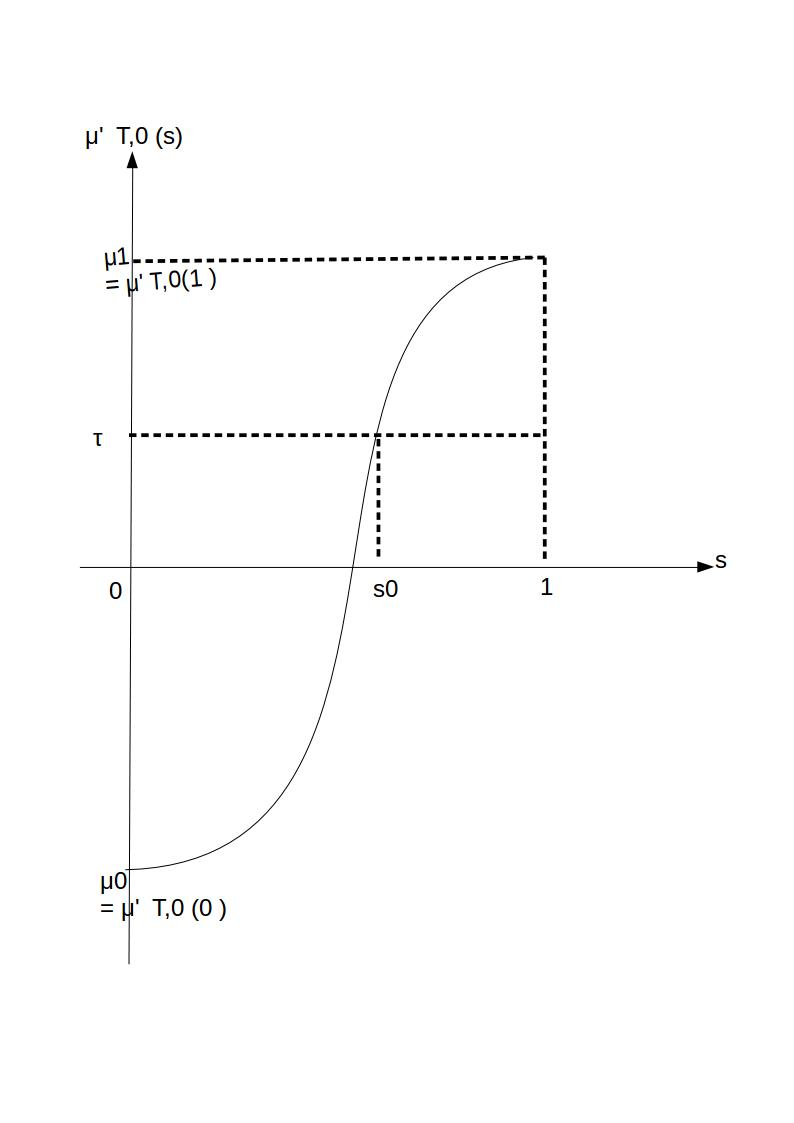
\includegraphics[scale=0.20]{Figures/Untitled1.jpg}
	\caption{variation of derivative of CGF of $T(y)$ with s. At $s_0$, $\tau$ is attained. \textit{(Source: H. Vincent Poor, An Introduction to Signal Detection and Estimation(Second Edition))}}
	\label{fn2}
\end{figure}
\begin{rem}
If $\tau\in(\mu_0,\mu_1)$ then, $\exists s_0\in[0,1]:f^\prime(s_0)=0$ \{KL divergence is the dual of $\log(MGF)$. Therefore, $\mathbb{E}_0\left[\log\left(\frac{P_1(y)}{P_0(y)}\right)\right]$ gives negative KL divergence.\}.
\end{rem}
We have,
\begin{align}\label{eqn:peb3}
&P_F(\tilde\delta_T)\leq e^{\mu_{T,0}(s_0)-s_0\mu\prime_{T,0}(s_0)},\\\label{eqn:peb4}
&P_M(\tilde\delta_T)\leq e^{\mu_{T,0}(s_0)+(1-s_0)\mu\prime_{T,0}(s_0)}.
\end{align}
This is called Chernoff bound technique.
\begin{note}
When $\tau\leq \mu_0$, $\mu^\prime_{T,0}(s)\geq \tau,\forall s\geq 0$, hence $f^\prime(s)\geq 0$. This means that $\min_{\forall s \geq 0}{f(s)}=f(0)$, and hence $P_F(\tilde\delta_T) \leq 1$.
\end{note}
\begin{note}
Similar to above, when $\tau\geq\mu_1$, we get, $P_M(\tilde\delta_T)\leq 1$.
\end{note}
\begin{exmp}\textbf{For Bayesian hypothesis testing:}
\par Assume prior probabilities are $\pi_0$ and $\pi_1$ (for $H_0$ and $H_1$), then average probability of error is,
\begin{align}\label{eqn:peb2}
&P_e=\pi_0P_F+\pi_1P_M,\nonumber\\
&P_e\leq\pi_0 e^{\mu_{T,0}(s_0)-s_0 \mu^\prime_{T,0}(s_0)}+\pi_1 e^{\mu_{T,0}(s_0)-(1-s_0) \mu^\prime_{T,0}(s_0)}.
\end{align}
Therefore,
\begin{equation}\label{eqn:peb1}
P_e\leq[\pi_0+\pi_1 e^{\mu^\prime{T,0}(s_0)}] e^{\mu_{T,0}(s_0)-s_0\mu^\prime_{T,0}(s_0)}
 \end{equation}
\eqref{eqn:peb1} is of the form $(A+B)C$ and inequality \eqref{eqn:peb2} is obtained from eqns. \eqref{eqn:peb3}, \eqref{eqn:peb4}. In fact, one can derive slightly tighter bound than bound obtained in \eqref{eqn:peb1},
\begin{equation}
P_e\leq \max\{\pi_0,\pi_1 e^{\mu^\prime_{T,0}(s_0)}\} e^{\mu_{T,0}(s_0)-s_0\mu^\prime_{T,0}(s_0)},~\forall~0\leq s_0\leq 1
\end{equation}
For the detector, $\log(L(y))\gtreqqless\tau$, recalling the minimum probability of error obtained for Bayesian decision rule assuming equal costs, we choose a threshold $\tau=\log\left(\frac{\pi_0}{\pi_1}\right)$. For this detector,
\begin{align*}
P_e&\leq\max\{\pi_0,\frac{\pi_0}{\pi_1}\cdot \pi_1\} e^{\mu_{T,0}(s)-s \log\left(\frac{\pi_0}{\pi_1}\right)},\\
&=\pi_0^{1-s}\cdot \pi_1^s\cdot e^{\mu_{T,0}(s)},~\forall~s\in [0,1].
\end{align*}
Therefore,
\begin{equation}
P_e\leq =\pi_0^{1-s}\cdot \pi_1^s e^{\mu_{T,0}(s)},\forall s\in [0,1]
\end{equation}
Hence, one can try and optimize RHS of above equation over $s$.
\end{exmp}
\begin{exmp}
\textbf{IID Observations:}
\par For $\Gamma\in \mathbb{R}^n$, and vector $Y=(y_1,y_2,\dots,y_n)\sim f_j$ under $H_j$ then,
\begin{align*}
\mu_{T,0}(s)&=\log\left(\mathbb{E}_0\left[e^{s\log(L(y))}\right]\right),\\
&=\log\left(\mathbb{E}_0\left[e^{s\log\left(\prod_{k=1}^n\frac{f_1(y_k)}{f_0(y_k)}\right)}\right],\right),\\
&=\log\left(\mathbb{E}_0\left[f_1^{s}(y) f_0^{-s}(y)\right]\right),\\
&= n\log\left(\int_{\Gamma}{f_1^{s}(y) f_0^{-s}(y) f_0(y)} dy\right),\\
&= n\log\left(\int_{\Gamma}{\left[\frac{f_1(y)}{f_0(y)}\right]^{s} f_0(y)} dy \right).
\end{align*}
Now,
\begin{align}
\int_{\Gamma}{\left[\frac{f_1(y)}{f_0(y)}\right]^{s} f_0(y)} dy =\mathbb{E}\left[\left(\frac{f_1(y)}{f_0(y)}\right)^s\right],
\end{align}
and,
\begin{align}
\mathbb{E}\left[\left(\frac{f_1(y)}{f_0(y)}\right)^s\right]\leq\left\{\mathbb{E}_0\left[\frac{f_1(y)}{f_0(y)}\right]\right\}^s
\end{align}
and we know, $\left\{\mathbb{E}_0\left[\frac{f_1(y)}{f_0(y)}\right]\right\}^s = 1$, therefore,
\begin{align*}
\mathbb{E}\left[\left(\frac{f_1(y)}{f_0(y)}\right)^s\right] &= n \log(a),~a<1\\
&= -n c,~c>0.
\end{align*}
\end{exmp}
\begin{note}
For minimum Probability of error Bayesian detector,
\begin{equation*}
P_e\leq \pi_0^{1-s}\cdot \pi_1^s e^{-n c(s)},~\forall s\in (0,1),
\end{equation*} 
here $c(s)$ should be positive. Probability of making an error decreases exponentially when $n$ increases.
\end{note}
\begin{note}
By Chernoff's theorem, optimal choice for $s\in(0,1)$ is given by,
\begin{equation*}
\max_{s\in (0,1)}{c(s)}=D(f||f_0)
\end{equation*}
where $\{f:D(f||f_0)=D(f||f_1)\}$.
\end{note}
\end{document}